% Standalone vector PDF of the opendrg OMOP CDM ER & output schema.
% Build: tectonic omop_er_schema.tex

\documentclass[tikz,border=16pt]{standalone}

\usepackage{ifxetex}
\ifxetex
  \usepackage{fontspec}
  \setmainfont{Times}
  \setsansfont{Helvetica}
\fi
\usepackage{amsmath}
\usepackage{xcolor}
\usetikzlibrary{arrows.meta,positioning,shapes.geometric,fit,backgrounds}

\definecolor{color1}{RGB}{59,80,114}
\definecolor{color2}{RGB}{0,20,20}

\begin{document}
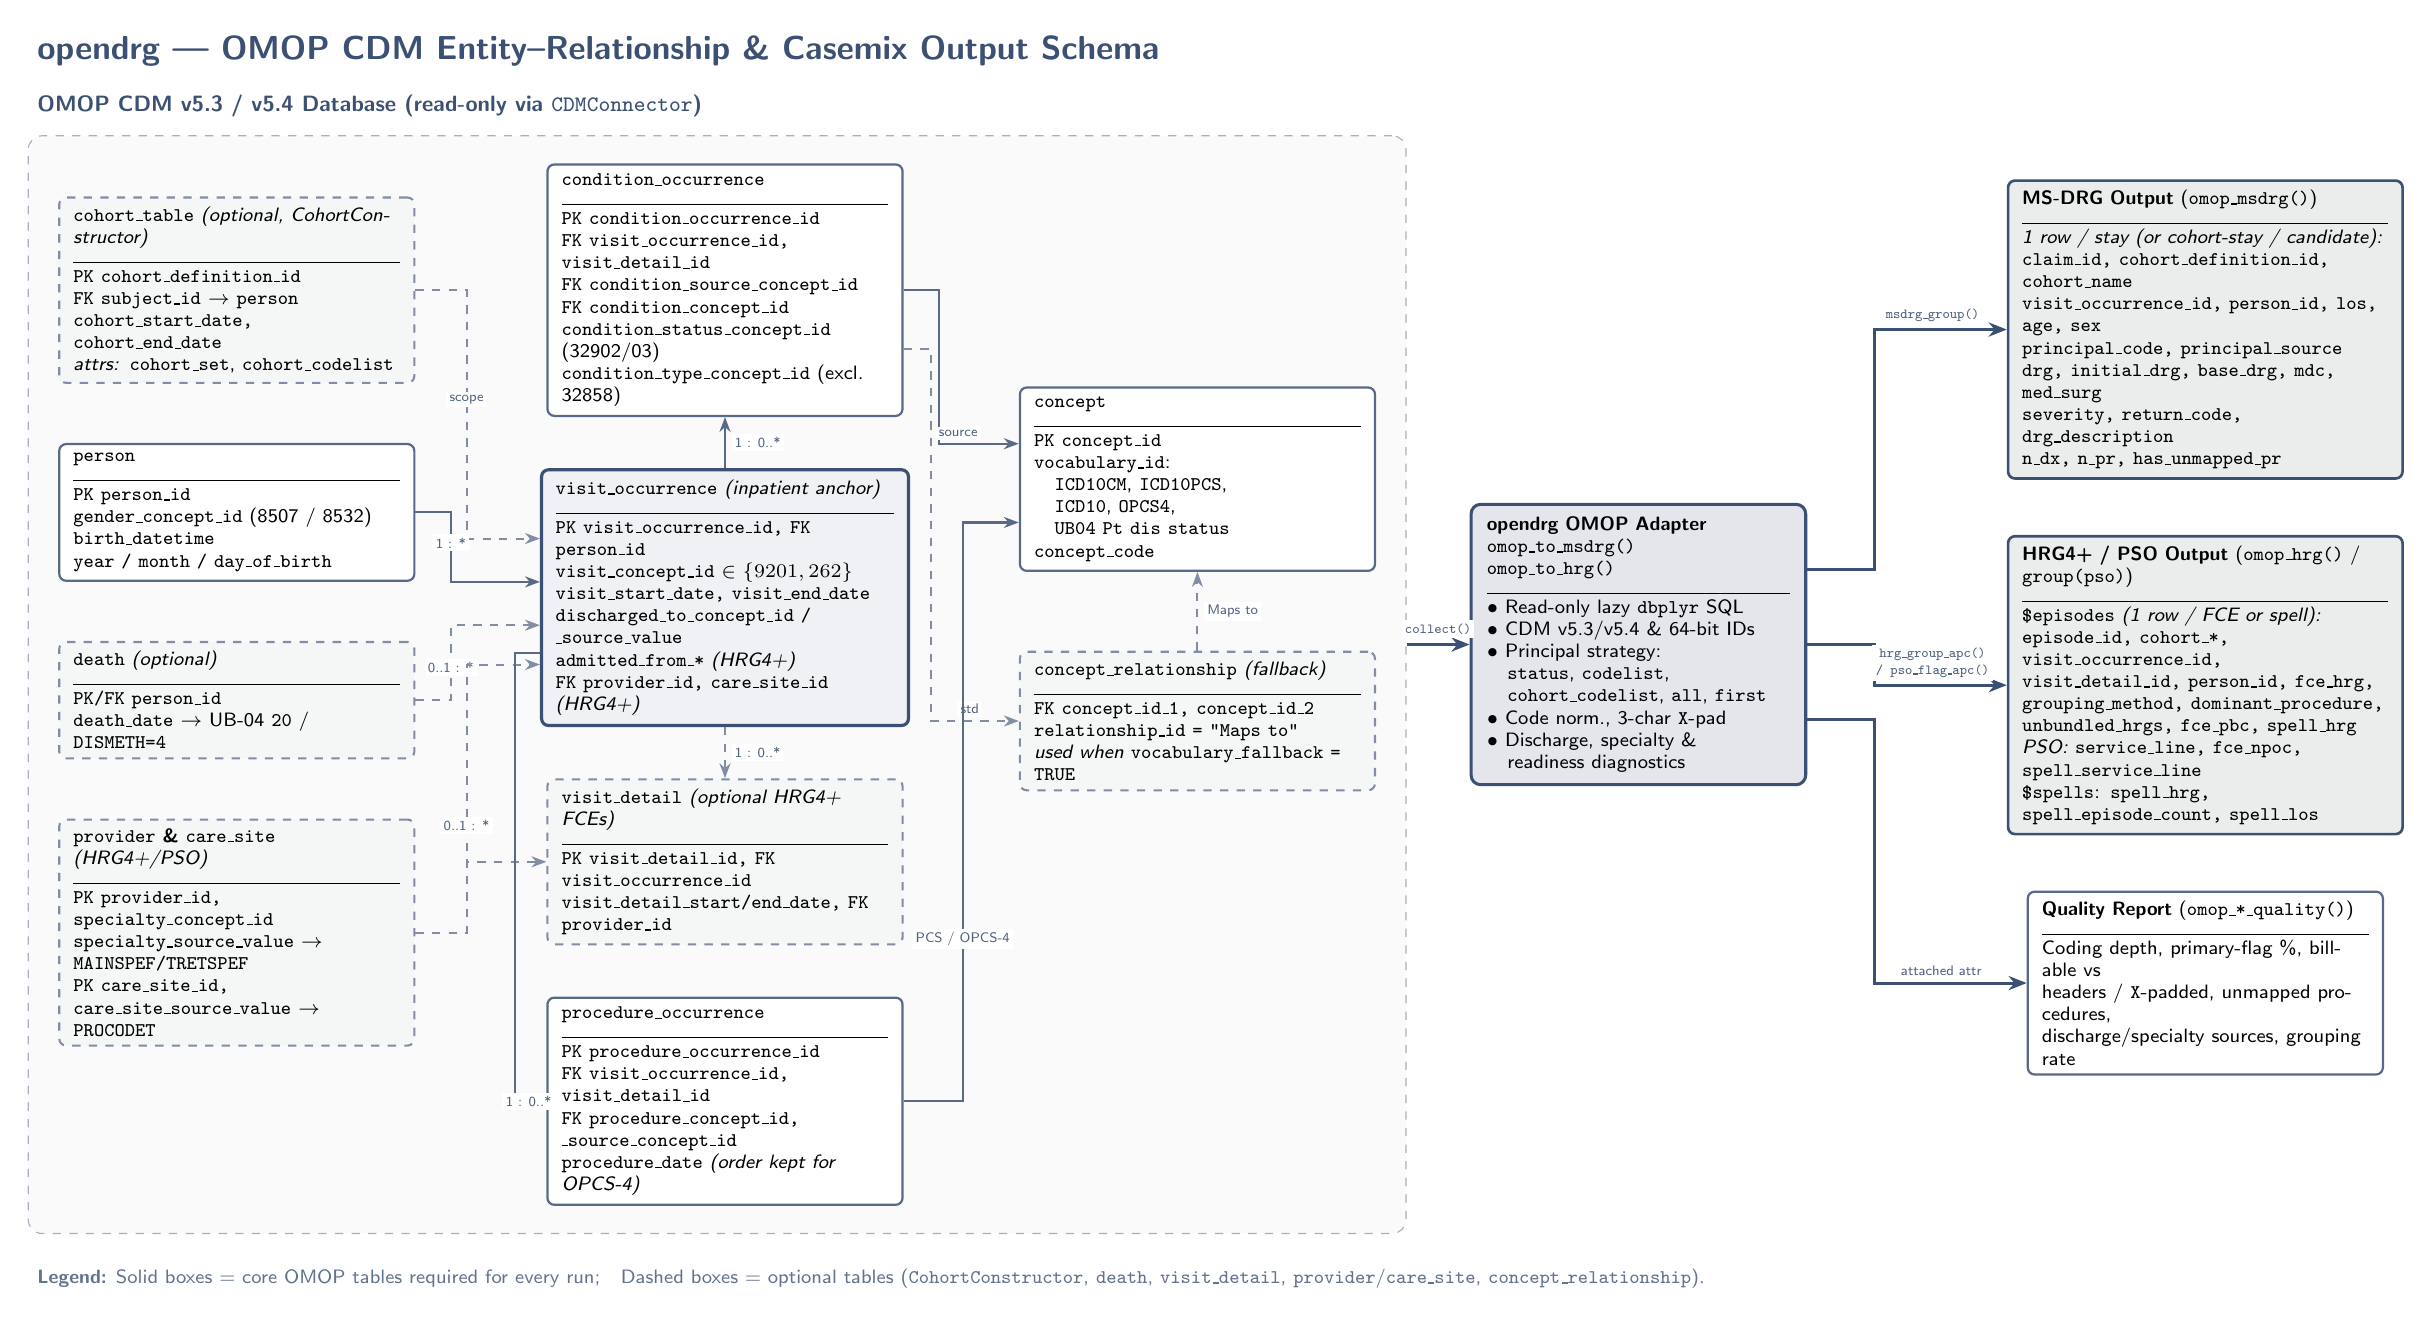
\begin{tikzpicture}[
    font=\sffamily\scriptsize,
    ent/.style={draw=color1!85, line width=0.8pt, rounded corners=2.5pt, fill=white, align=left, inner xsep=0.18cm, inner ysep=0.12cm, text width=4.15cm},
    entopt/.style={draw=color1!65, dashed, line width=0.75pt, rounded corners=2.5pt, fill=color2!4, align=left, inner xsep=0.18cm, inner ysep=0.12cm, text width=4.15cm},
    anchorbox/.style={draw=color1, line width=1.15pt, rounded corners=2.5pt, fill=color1!8, align=left, inner xsep=0.18cm, inner ysep=0.13cm, text width=4.3cm},
    adapter/.style={draw=color1, line width=1.1pt, rounded corners=3.5pt, fill=color1!14, align=left, inner xsep=0.2cm, inner ysep=0.16cm, text width=3.85cm},
    outbox/.style={draw=color1, line width=0.95pt, rounded corners=2.5pt, fill=color2!8, align=left, inner xsep=0.18cm, inner ysep=0.12cm, text width=4.65cm},
    rel/.style={-{Stealth[length=1.9mm,width=1.4mm]}, line width=0.75pt, color=color1!85},
    relopt/.style={-{Stealth[length=1.9mm,width=1.4mm]}, dashed, line width=0.7pt, color=color1!65},
    flow/.style={-{Stealth[length=2.3mm,width=1.8mm]}, line width=1.05pt, color=color1},
    lbl/.style={font=\sffamily\tiny, fill=white, inner sep=1.2pt, text=color1!90}
]

% --- Column 2 (x = 6.2): Core Visits & Clinical Events ---
\node[ent] (cond) at (6.2, 4.6) {%
  \textbf{\texttt{condition\_occurrence}}\\[-1pt]
  \rule{\linewidth}{0.35pt}\\[-1pt]
  \texttt{PK condition\_occurrence\_id}\\
  \texttt{FK visit\_occurrence\_id, visit\_detail\_id}\\
  \texttt{FK condition\_source\_concept\_id}\\
  \texttt{FK condition\_concept\_id}\\
  \texttt{condition\_status\_concept\_id} (32902/03)\\
  \texttt{condition\_type\_concept\_id} (excl.\ 32858)%
};

\node[anchorbox, below=0.65cm of cond] (visit) {%
  \textbf{\texttt{visit\_occurrence}} \textit{(inpatient anchor)}\\[-1pt]
  \rule{\linewidth}{0.45pt}\\[-1pt]
  \texttt{PK visit\_occurrence\_id, FK person\_id}\\
  \texttt{visit\_concept\_id} $\in \{9201, 262\}$\\
  \texttt{visit\_start\_date, visit\_end\_date}\\
  \texttt{discharged\_to\_concept\_id / \_source\_value}\\
  \texttt{admitted\_from\_*} \textit{(HRG4+)}\\
  \texttt{FK provider\_id, care\_site\_id} \textit{(HRG4+)}%
};

\node[entopt, below=0.65cm of visit] (vdet) {%
  \textbf{\texttt{visit\_detail}} \textit{(optional HRG4+ FCEs)}\\[-1pt]
  \rule{\linewidth}{0.35pt}\\[-1pt]
  \texttt{PK visit\_detail\_id, FK visit\_occurrence\_id}\\
  \texttt{visit\_detail\_start/end\_date, FK provider\_id}%
};

\node[ent, below=0.65cm of vdet] (proc) {%
  \textbf{\texttt{procedure\_occurrence}}\\[-1pt]
  \rule{\linewidth}{0.35pt}\\[-1pt]
  \texttt{PK procedure\_occurrence\_id}\\
  \texttt{FK visit\_occurrence\_id, visit\_detail\_id}\\
  \texttt{FK procedure\_concept\_id, \_source\_concept\_id}\\
  \texttt{procedure\_date} \textit{(order kept for OPCS-4)}%
};

% --- Column 1 (x = 0): Patient, Cohort, Death, Admin ---
\node[entopt] (cohort) at (0, 4.6) {%
  \textbf{\texttt{cohort\_table}} \textit{(optional, CohortConstructor)}\\[-1pt]
  \rule{\linewidth}{0.35pt}\\[-1pt]
  \texttt{PK cohort\_definition\_id}\\
  \texttt{FK subject\_id} $\rightarrow$ \texttt{person}\\
  \texttt{cohort\_start\_date, cohort\_end\_date}\\
  \textit{attrs:} \texttt{cohort\_set}, \texttt{cohort\_codelist}%
};

\node[ent, below=0.75cm of cohort] (person) {%
  \textbf{\texttt{person}}\\[-1pt]
  \rule{\linewidth}{0.35pt}\\[-1pt]
  \texttt{PK person\_id}\\
  \texttt{gender\_concept\_id} (8507 / 8532)\\
  \texttt{birth\_datetime}\\
  \texttt{year / month / day\_of\_birth}%
};

\node[entopt, below=0.75cm of person] (death) {%
  \textbf{\texttt{death}} \textit{(optional)}\\[-1pt]
  \rule{\linewidth}{0.35pt}\\[-1pt]
  \texttt{PK/FK person\_id}\\
  \texttt{death\_date} $\rightarrow$ UB-04 \texttt{20} / \texttt{DISMETH=4}%
};

\node[entopt, below=0.75cm of death] (admin) {%
  \textbf{\texttt{provider} \& \texttt{care\_site}} \textit{(HRG4+/PSO)}\\[-1pt]
  \rule{\linewidth}{0.35pt}\\[-1pt]
  \texttt{PK provider\_id, specialty\_concept\_id}\\
  \texttt{specialty\_source\_value} $\rightarrow$ \texttt{MAINSPEF/TRETSPEF}\\
  \texttt{PK care\_site\_id, care\_site\_source\_value} $\rightarrow$ \texttt{PROCODET}%
};

% --- Column 3 (x = 12.2): OMOP Vocabularies (inside OMOP CDM box) ---
\node[ent] (concept) at (12.2, 2.2) {%
  \textbf{\texttt{concept}}\\[-1pt]
  \rule{\linewidth}{0.35pt}\\[-1pt]
  \texttt{PK concept\_id}\\
  \texttt{vocabulary\_id}:\\
  \quad\texttt{ICD10CM}, \texttt{ICD10PCS},\\
  \quad\texttt{ICD10}, \texttt{OPCS4},\\
  \quad\texttt{UB04 Pt dis status}\\
  \texttt{concept\_code}%
};

\node[entopt, below=1.0cm of concept] (crel) {%
  \textbf{\texttt{concept\_relationship}} \textit{(fallback)}\\[-1pt]
  \rule{\linewidth}{0.35pt}\\[-1pt]
  \texttt{FK concept\_id\_1, concept\_id\_2}\\
  \texttt{relationship\_id = "Maps to"}\\
  \textit{used when} \texttt{vocabulary\_fallback = TRUE}%
};

% --- Background grouping box strictly around OMOP CDM tables ---
\begin{pgfonlayer}{background}
  \node[draw=color1!45, dashed, rounded corners=5pt, fill=color2!2, inner xsep=0.38cm, inner ysep=0.35cm,
        fit=(cohort)(person)(death)(admin)(cond)(visit)(vdet)(proc)(concept)(crel)] (cdmbox) {};
  \node[anchor=south west, font=\sffamily\bfseries\footnotesize, text=color1] at ([yshift=3pt]cdmbox.north west)
        {OMOP CDM v5.3 / v5.4 Database (read-only via \texttt{CDMConnector})};
\end{pgfonlayer}

% --- Column 4 (x = 17.8): opendrg OMOP Adapter ---
\node[adapter] (adapter) at (17.8, 0.1) {%
  \textbf{opendrg OMOP Adapter}\\
  \texttt{omop\_to\_msdrg()}\\
  \texttt{omop\_to\_hrg()}\\[-1pt]
  \rule{\linewidth}{0.45pt}\\[-1pt]
  $\bullet$ Read-only lazy \texttt{dbplyr} SQL\\
  $\bullet$ CDM v5.3/v5.4 \& 64-bit IDs\\
  $\bullet$ Principal strategy:\\
  \quad\texttt{status}, \texttt{codelist},\\
  \quad\texttt{cohort\_codelist}, \texttt{all}, \texttt{first}\\
  $\bullet$ Code norm., 3-char \texttt{X}-pad\\
  $\bullet$ Discharge, specialty \&\\
  \quad readiness diagnostics%
};

% --- Column 5 (x = 25.0): Grouped Outputs ---
\node[outbox] (out_msdrg) at (25.0, 4.1) {%
  \textbf{MS-DRG Output} (\texttt{omop\_msdrg()})\\[-1pt]
  \rule{\linewidth}{0.4pt}\\[-1pt]
  \textit{1 row / stay (or cohort-stay / candidate):}\\
  \texttt{claim\_id, cohort\_definition\_id, cohort\_name}\\
  \texttt{visit\_occurrence\_id, person\_id, los, age, sex}\\
  \texttt{principal\_code, principal\_source}\\
  \texttt{drg, initial\_drg, base\_drg, mdc, med\_surg}\\
  \texttt{severity, return\_code, drg\_description}\\
  \texttt{n\_dx, n\_pr, has\_unmapped\_pr}%
};

\node[outbox, below=0.7cm of out_msdrg] (out_hrg) {%
  \textbf{HRG4+ / PSO Output} (\texttt{omop\_hrg()} / \texttt{group(pso)})\\[-1pt]
  \rule{\linewidth}{0.4pt}\\[-1pt]
  \textbf{\texttt{\$episodes}} \textit{(1 row / FCE or spell):}\\
  \texttt{episode\_id, cohort\_*, visit\_occurrence\_id,}\\
  \texttt{visit\_detail\_id, person\_id, fce\_hrg,}\\
  \texttt{grouping\_method, dominant\_procedure,}\\
  \texttt{unbundled\_hrgs, fce\_pbc, spell\_hrg}\\
  \textit{PSO:} \texttt{service\_line, fce\_npoc, spell\_service\_line}\\
  \textbf{\texttt{\$spells}}: \texttt{spell\_hrg, spell\_episode\_count, spell\_los}%
};

\node[ent, below=0.7cm of out_hrg] (out_qual) {%
  \textbf{Quality Report} (\texttt{omop\_*\_quality()})\\[-1pt]
  \rule{\linewidth}{0.35pt}\\[-1pt]
  Coding depth, primary-flag \%, billable vs\\
  headers / \texttt{X}-padded, unmapped procedures,\\
  discharge/specialty sources, grouping rate%
};

% --- ER Relationships (Col 1 -> Col 2) ---
\draw[relopt] (cohort.east) -- ++(0.65,0) |- node[lbl, pos=0.22] {scope} ([yshift=0.75cm]visit.west);
\draw[rel] (person.east) -- ++(0.45,0) |- node[lbl, pos=0.22] {1 : *} ([yshift=0.2cm]visit.west);
\draw[relopt] (death.east) -- ++(0.45,0) |- node[lbl, pos=0.22] {0..1 : *} ([yshift=-0.35cm]visit.west);
\draw[relopt] (admin.east) -- ++(0.65,0) |- node[lbl, pos=0.2] {0..1 : *} ([yshift=-0.85cm]visit.west);
\draw[relopt] (admin.east) -- ++(0.65,0) |- (vdet.west);

% --- ER Relationships (within Col 2) ---
\draw[rel] (visit.north) -- node[lbl, right=2pt] {1 : 0..*} (cond.south);
\draw[relopt] (visit.south) -- node[lbl, right=2pt] {1 : 0..*} (vdet.north);
\draw[rel] ([yshift=-0.7cm]visit.west) -- ++(-0.32,0) |- node[lbl, pos=0.72] {1 : 0..*} (proc.west);

% --- Vocabulary joins (Col 2 -> Col 3) ---
\draw[rel] (cond.east) -- ++(0.45,0) |- node[lbl, pos=0.62, above=1pt] {source} ([yshift=0.45cm]concept.west);
\draw[relopt] ([yshift=-0.75cm]cond.east) -- ++(0.35,0) |- node[lbl, pos=0.72, above=1pt] {std} (crel.west);
\draw[relopt] (crel.north) -- node[lbl, right=2pt] {Maps to} (concept.south);
\draw[rel] (proc.east) -- ++(0.75,0) |- node[lbl, pos=0.14] {PCS / OPCS-4} ([yshift=-0.55cm]concept.west);

% --- CDM Box -> Adapter ---
\draw[flow] (cdmbox.east |- adapter.west) -- node[lbl, above=2pt] {\texttt{collect()}} (adapter.west);

% --- Adapter -> Outputs ---
\draw[flow] ([yshift=0.95cm]adapter.east) -- ++(0.85,0) |- node[lbl, pos=0.72, above=1pt] {\texttt{msdrg\_group()}} (out_msdrg.west);
\draw[flow] ([yshift=0.0cm]adapter.east) -- ++(0.85,0) |- node[lbl, align=center, pos=0.72, above=1pt] {\texttt{hrg\_group\_apc()}\\ \texttt{/ pso\_flag\_apc()}} (out_hrg.west);
\draw[flow] ([yshift=-0.95cm]adapter.east) -- ++(0.85,0) |- node[lbl, pos=0.72, above=1pt] {attached attr} (out_qual.west);

% --- Title & Legend ---
\node[anchor=south west, font=\sffamily\bfseries\large, text=color1] at ([yshift=0.75cm]cdmbox.north west)
  {opendrg --- OMOP CDM Entity--Relationship \& Casemix Output Schema};
\node[anchor=north west, font=\sffamily\scriptsize, text=color1!80] at ([yshift=-0.32cm]cdmbox.south west)
  {\textbf{Legend:} Solid boxes = core OMOP tables required for every run;\quad Dashed boxes = optional tables (\texttt{CohortConstructor}, \texttt{death}, \texttt{visit\_detail}, \texttt{provider}/\texttt{care\_site}, \texttt{concept\_relationship}).};

\end{tikzpicture}
\end{document}
